\chapter{Sviluppo applicazione}\label{c:applicazione}

L'applicazione che è stata sviluppata ha lo scopo di fornire un supporto per gli utenti interessati agli investimenti in aziende e start up, usando algoritmi di machine learning per predire l'andamento futuro di un'azienda, sulla base di alcuni dati rappresentativi dell'azienda specifica. 

È stato deciso di sviluppare un'applicazione desktop in linguaggio Python perchè il più adatto per la gestione dei dati e la loro manipolazione prima di essere usati per algoritmi di machine learning, e data la piena compatibilità con le API di PredictionIO per l'interazione con l'event server e i vari engines. Infatti la parte di machine learning è gestita interamente da PredictionIO. Mentre per l'interfaccia grafica è stata usata la libreria TKinter di Python, la libreria grafica standard per questo linguaggio.

Di seguito sarà illustrato come è stata sviluppata l'applicazione, come è stato usato PredictionIO e come si integra con l'applicazione.

\section{Funzionalità e scopo}
L'applicazione sviluppata consente di creare un account personale inserendo i propri dati, con il quale sarà poi possibile cercare aziende presenti nell'applicazione e vederne i principali dati, salvare nei preferiti quelle che interessano di più e poter fare una previsione sull'andamento futuro dell'azienda e quindi sulla convenienza di investimento. 

\begin{figure}[!h]
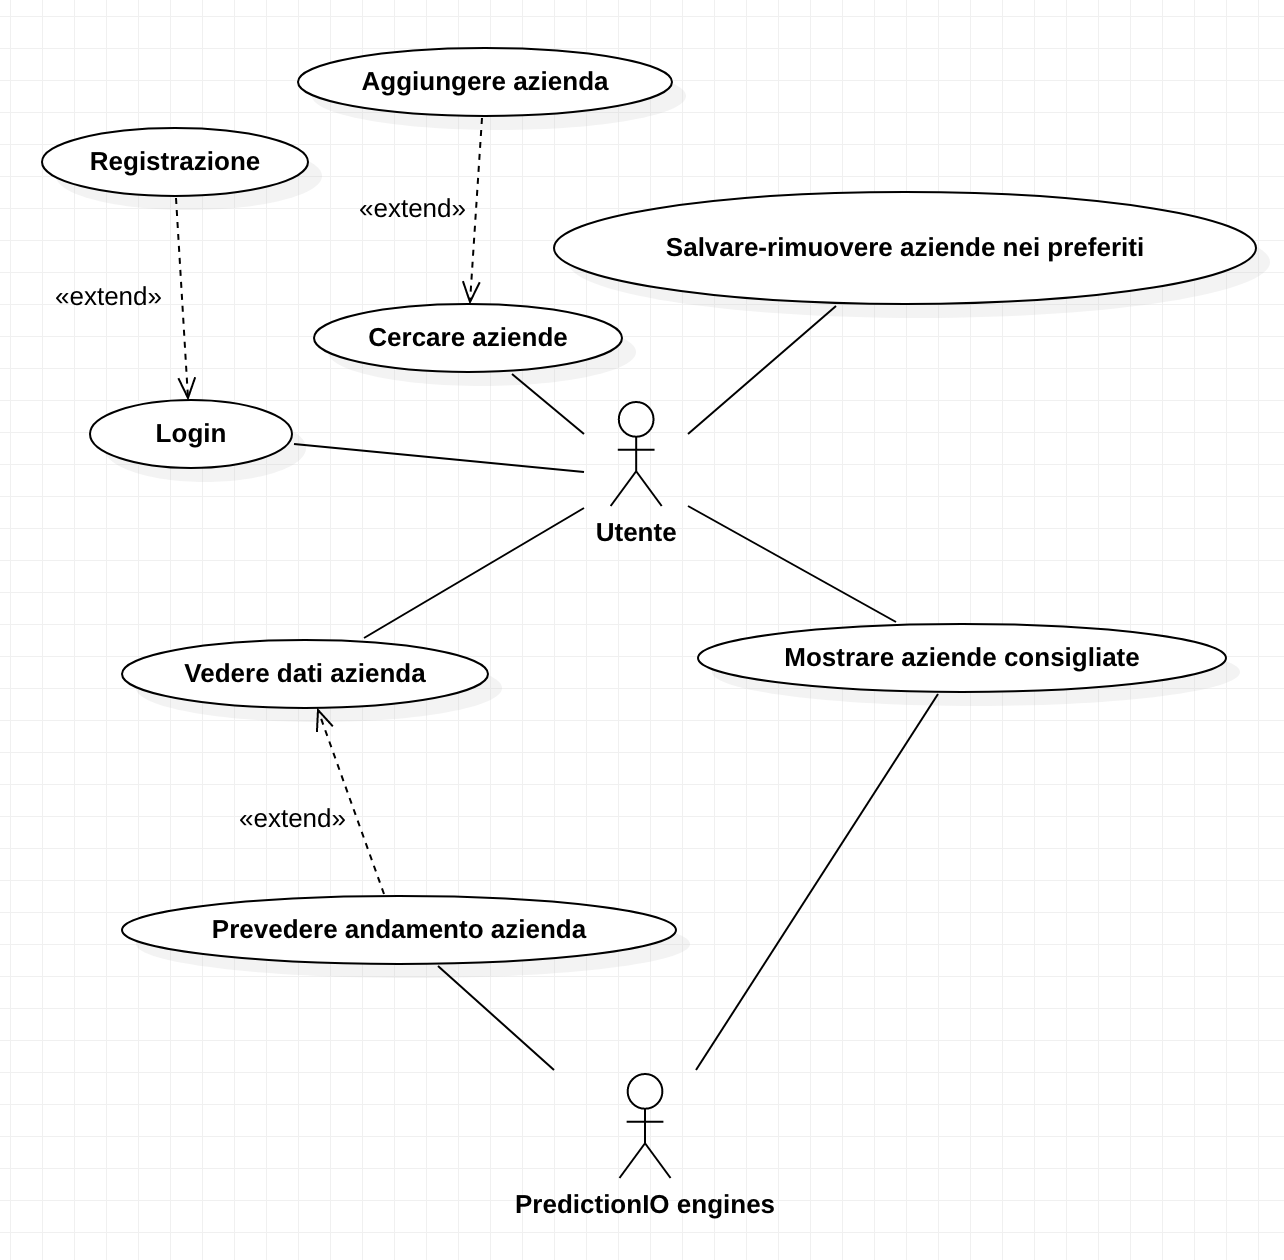
\includegraphics[width=1.0\textwidth]{immagini/usecase.png}
\caption{Use Case Diagram}
\label{fig:usecase}
\end{figure}

\section{Struttura dell'applicazione}
L'applicazione si compone di diversi moduli rappresentati da classi Python. Alcuni moduli rappresentano delle schermate dell'applicazione, ognuna con una funzionalità diversa:
\begin{itemize}
\item \textbf{Schermata di login}: è la prima schermata mostrata quando si avvia l'applicazione e semplicemente consente di effettuare il login inserendo \textit{username} e \textit{password}.
\item \textbf{Schermata di registrazione}: se non si ha già un account, dalla schermata di login è possibile spostarsi nella schermata di registrazione per creare un nuovo account inserendo i propri dati.
\item \textbf{Schermata di home page}: è la schermata principale che compare quando si effettua il login e nella quale sono presenti tre sezioni principali:
\begin{itemize}
\item \textbf{Preferiti}: nella quale vengono mostrate le aziende salvate come preferite da quell'utente.
\item \textbf{Consigliati}: nella quale vengono mostrate delle aziende consigliate in base alle preferenze di quell'utente. Questa lista viene creata usando un algoritmo di machine learning di recommendation, implementato in un engine di PredictionIO (si veda  \ref{subsubsec:racc}).
\item \textbf{Ricerca}: nella quale si possono effettuare delle ricerche specificando il nome dell'azienda che si vuole trovare.
\end{itemize}
\item \textbf{Profilo}: è la schermata nella quale è possibile modificare i dati del proprio account, come username, nome e cognome, o fare la reimpostazione della password.
\item \textbf{Azienda}: è la schermata che descrive l'azienda, mostrando i dati principali e nella quale è possibile salvare nei preferiti quell'azienda, o toglierla dai preferiti nel caso fosse già salvata. Inoltre è possibile richiedere una previsione sul futuro andamento dell'azienda con dei relativi consigli sull'investimento, questo è possibile grazie a un algoritmo di machine learning di classificazione, il RandomForest, implementato in un engine di PredictionIO (si veda \ref{subsubsec:class}).
\item \textbf{Inserimento azienda}: se un'azienda non è presente e non viene trovata con una ricerca è possibile aggiungerla inserendo i dati richiesti.
\end{itemize}

Altri moduli fondamentali sono la \textbf{Main Page}, che ha il compito di gestire le varie schermate e le transizioni tra esse. Il \textbf{DBManager} che gestisce il database, consentendo di modificare i dati aggiungendo o modificando utenti nella fase di iscrizione o quando si modificano i propri dati. Il \textbf{Predictor} infine è il modulo che gestisce le parti di machine learning e quindi è dove è implementata l'integrazione con gli engines di PredictionIO.

Le classi che rappresentano i moduli di cui sopra sono rappresentate dal seguente class diagram.

\newpage

\begin{figure}[!h]
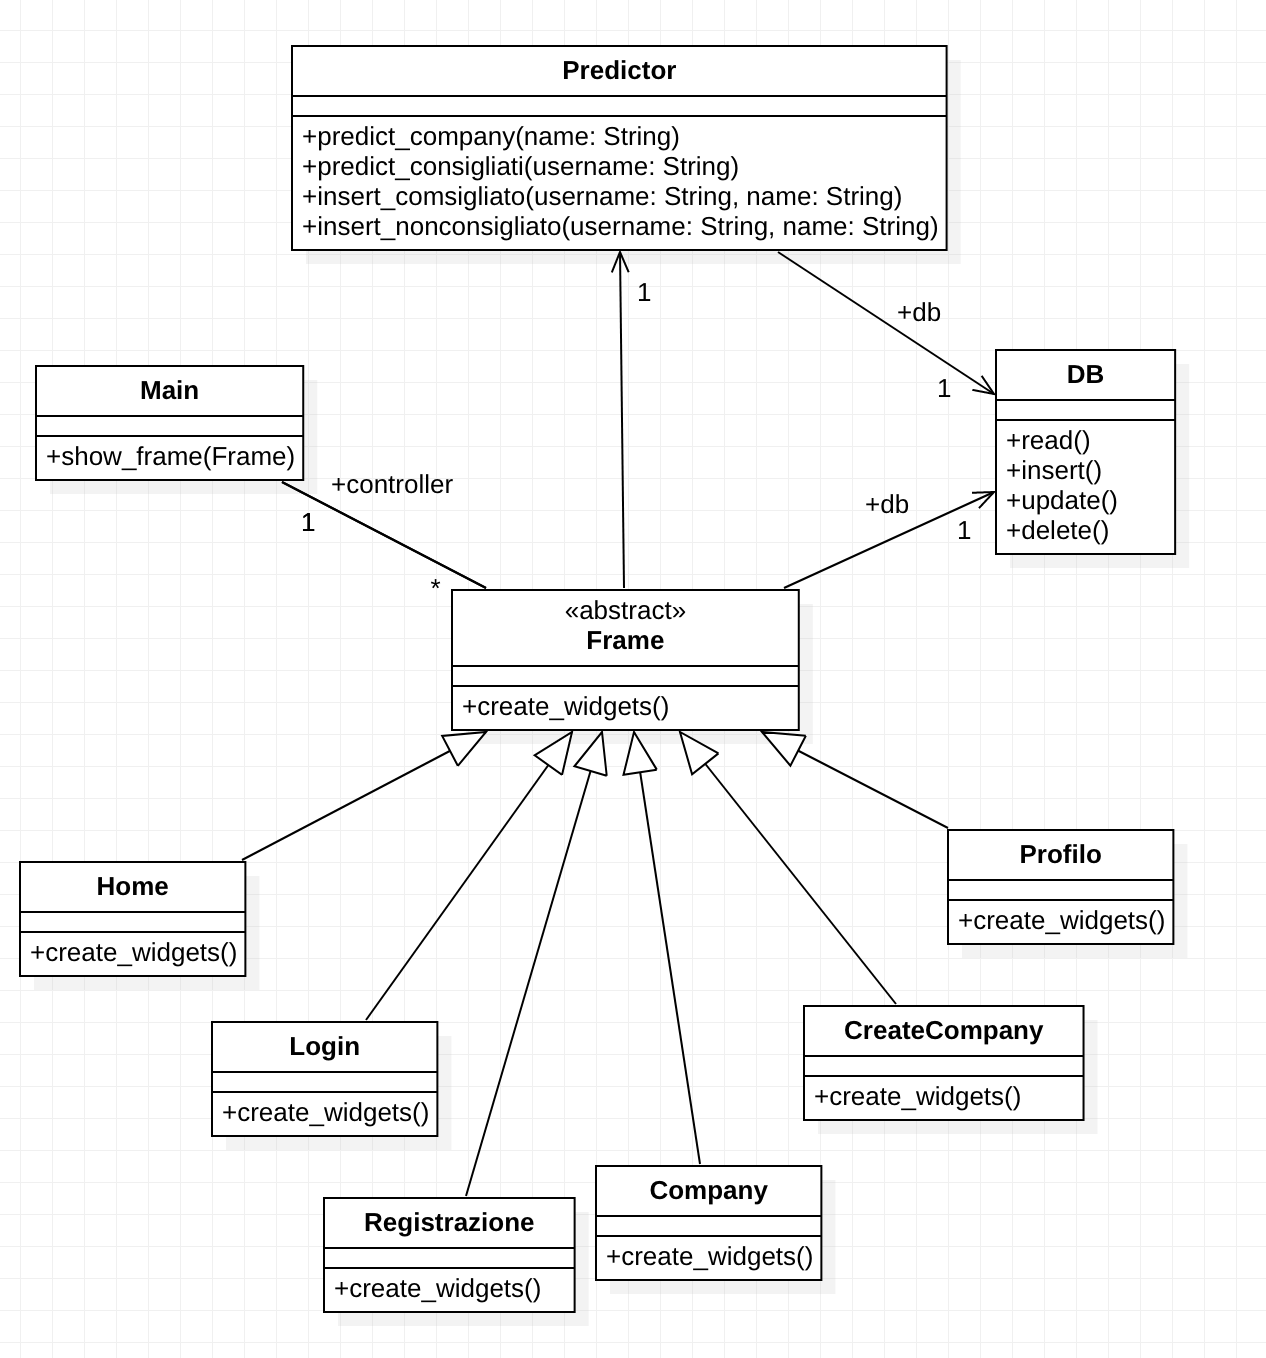
\includegraphics[width=1.0\textwidth]{immagini/classdiagram.png}
\caption{Class Diagram}
\label{fig:classdiagram}
\end{figure}

In particolare la classe \textbf{Frame} è la classe madre di tutti i moduli che rappresentano delle schermate, ogni implementazione concreta sovrascriverà il metodo \verb+create_widgets()+ che ha lo scopo di creare gli elementi visivi presenti e posizionarli sulla schermata di riferimento con le dovute dimensioni e distanze tra essi. Di seguito un esempio di metodo \verb+create_widgets()+ della classe LoginPage, che rappresenta la schermata di login. 

\begin{figure}[!h]
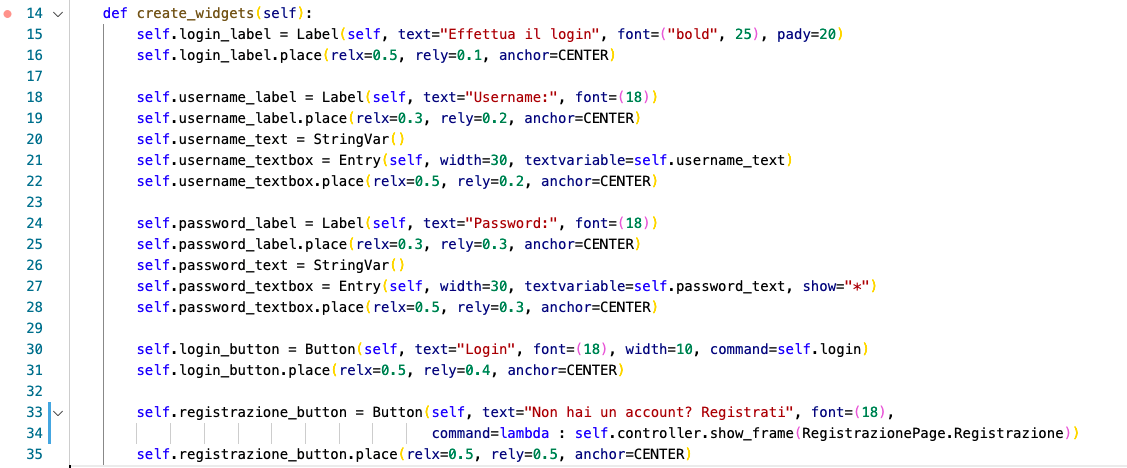
\includegraphics[width=1.0\textwidth]{immagini/createwidgets.png}
\caption{Metodo create\_widgets() di LoginPage \cite{codice}}
\label{fig:createwidgets}
\end{figure}

Inoltre l'attributo \verb+controller+ è di tipo MainPage e si riferisce all'oggetto MainPage che ha creato quello specifico Frame, il quale sarà utilizzato per chiamare il metodo \verb+show_frame()+ per cambiare schermata.

La classe \textbf{MainPage} ha lo scopo di gestire le schermate e le loro transizioni, e lo fa con il metodo \verb+show_frame(Frame)+, in particolare questa classe ha una lista di oggetti Frame che rappresentano tutte le varie schermate dell'applicazione, e quando questo metodo viene invocato esso mostra il Frame che gli è stato passato come parametro mentre elimina tutti gli altri, in questo modo viene cambiata la schermata mostrata a video.

\section{Database}
La classe che gestisce la connessione al database è \textbf{DB}, e quando viene istanziata si connette al database usando i parametri definiti in un file di configurazione che deve essere presente e avere il seguente formato:
\newpage
\begin{verbatim}
host=localhost
database=nomedb
user=nomeuser
password=password
\end{verbatim}
La classe DB si collegherà a questo database e, se non sono già presenti, creerà le seguenti tabelle:
\begin{itemize}
\item \textbf{users}: rappresenta tutti gli utenti registrati all'applicazione, i quali sono descritti da diversi attributi:
\begin{itemize}
\item username: è la primary key e rappresenta quindi l'identificatore unico di ogni utente, viene usato per fare il login
\item nome
\item cognome
\item password
\end{itemize}
\item \textbf{companies}: è la tabella delle aziende disponibili nell'applicazione, descritte dagli attributi:
\begin{itemize}
\item nome: è la primary key, quindi è unica per ogni azienda ed è il nome legale dell'azienda
\item market: rappresenta il settore di mercato in cui l'azienda opera
\item total\_investment: è il totale in dollari di investimenti che l'azienda ha ricevuto nel corso della sua vita
\item funding\_rounds: è il numero di investimenti totali ricevuti, cioè quante volte si è investito nella azienda a prescindere dalla somma di denaro
\item founded\_at: rappresenta la data in cui è stata fondata
\item first\_funding\_at: rappresenta la data in cui ha ricevuto il primo investimento, questo attributo servirà per calcolare dei dati derivati per l'algoritmo di machine learning per la predizione dell'andamento (si veda \ref{subsubsec:class})
\item last\_funding\_at: rappresenta la data dell'ultimo investimento ricevuto, e come l'attributo \textit{first\_funding\_at} serve per calcolare dei dati derivati (si veda \ref{subsubsec:class})
\end{itemize}
\item \textbf{interested}: è la tabella che descrive gli interessi di tutti gli utenti, cioè quali aziende sono nei preferiti di ogni utente, gli attributi sono due e sono delle foreign key che si riferiscono alle entità user e company:
\begin{itemize}
\item username: primary key dell'utente
\item nome: primary key dell'azienda che l'utente descritto dallo username ha inserito nei preferiti
\end{itemize}
\end{itemize}

La classe DB ha dei metodi per la lettura, scrittura, modifica e eliminazione di queste tabelle, grazie ai quali le classi che rappresentano le schermate possono agire sul database per leggere i dati o effettuare delle modifiche. In questo modo tutta la complessità dell'accesso al database è incapsulata nella classe DB e le altre classi devono solo interagire con l'interfaccia che essa espone. Per lo sviluppo dell'applicazione è stato deciso di usare \textbf{MySQL} come DBMS e farlo girare in locale, ma in caso di modifica del DBMS basterà modificare la classe DB.

Tutte le classi che rappresentano delle schermate interagiscono con il database tramite la classe DB, tranne la classe Company. La classe Login controlla che esista l'utente e che la password inserita dall'utente in fase di accesso sia corretta, altrimenti mostrerà un messaggio di errore. La classe Registrazione controlla che lo username inserito dall'utente non esista già nel database, e nel caso non esista e gli attributi che descrivono l'utente siano stati inseriti nel modo corretto, registra il nuovo utente aggiungendolo alla tabella \textit{users}. La classe CreateCompany esegue la registrazione analoga a quella fatta dalla classe Registrazione ma per le aziende, quindi accedendo alla tabella \textit{companies}. La classe Profilo accede al database per aggiornare i dati modificati dall'utente.  Infine la classe Home accede al database in caso l'utente effettui una ricerca, quindi eseguirà una lettura nella tabella \textit{companies}, se esiste mostra l'azienda cercata altrimenti mostrerà un messaggio che inviterà l'utente ad aggiungere l'azienda non presente.

\section{Integrazione con PredictionIO}
La classe \textbf{Predictor} gestisce la parte di machine learning e fornisce quindi l'interfaccia con cui accedere agli engines di PredictionIO, manderà le query per fare una richiesta ai modelli e riceverà le risposte. Le richieste e le risposte saranno in un certo formato, quindi questa classe ha anche il compito di convertirle nelle varie forme richieste. I metodi principali della classe Predictor sono:
\begin{itemize}
\item \verb+predict_company(nome)+: ha il compito di mandare la richiesta di predire l'andamento futuro dell'azienda passata come parametro all'engine che implementa il modello di classificazione, per farlo deve accedere al database per leggere tutti gli attributi riferiti a quell'azienda.
\item \verb+transform_features(features)+: è il metodo tramite il quale \\ \verb+predict_company()+ converte gli attributi nel formato corretto per l'engine di PredictionIO, gli attributi da convertire sono passati come parametro sotto forma di lista Python. 
\item \verb+predict_consigliati(username)+: è il metodo che interagisce con l'engine che implementa il modello di raccomandazione, esegue una richiesta per avere 30 aziende consigliate all'utente passato come parametro.
\item \verb+insert_consigliato(username, nome)+: quando un utente salva nei preferiti un'azienda questo metodo invia all'event server questo evento, di tipo "interested", che descrive l'interesse dell'utente \textit{username} per l'azienda \textit{nome}. L'evento inviato sarà relativo al modello di raccomandazione, in questo modo l'engine potrà continuare il suo addestramento e fornire consigli più precisi.
\item \verb+insert_nonconsigliato(username, nome)+: è il metodo duale di \\ \verb+insert_consigliato()+, però manda un evento di tipo "not interested", cioè quando l'utente \textit{username} toglie dai preferiti l'azienda \textit{nome}, il che significa che non è più interessato.
\end{itemize}

Per interagire con gli engines la classe Predictor sfrutta le API di PredictionIO per Python, importando il modulo \verb+predictionio+ si potrà istanziare degli oggetti di tipo \verb+EngineClient+ e \verb+EventClient+, i primi per comunicare con gli engine, mandare richieste e ricevere risposte, mentre i secondi per mandare dati sotto forma di eventi all'event server. Di seguito due esempi di utilizzo:
\begin{verbatim}
import predictionio
engine_client = predictionio.EngineClient(url="http://localhost:8000")
event_client = predictionio.EventClient(access_key="access_key", 
 url="http://localhost:7070")

result = engine_client.send_query(query)

event_client.create_event(event="interested", entity_type="user", 
 entity_id=username, target_entity_type="company",
 target_entity_id=nome)
\end{verbatim}

La classe Predictor utilizza un oggetto di tipo \verb+EventClient+ per comunicare con l'event server e distinguerà gli engine passando come parametro le diverse access key, mentre utilizza due oggetti di tipo \verb+EngineClient+, ognuno istanziato per un solo engine.

\subsection{Formato delle richieste e risposte}
Le richieste agli engines devono essere in un certo formato per poter essere comprese, e a loro volta le risposte avranno lo stesso formato, la classe Predictor effettua le dovute conversioni. Il formato è il JSON, in particolare in Python viene usata la struttura dati \textit{dizionario}, cioè un insieme di coppie chiave-valore. 

Nel caso del modello di classificazione il metodo \verb+send_query()+ dell'oggetto \verb+EngineClient+ visto sopra accetta come parametro un dizionario, che avrà come chiavi i nomi delle features accettate dal modello, e come valori i corrispondenti valori delle features. Il risultato che restituisce sarà a sua volta un dizionario con il valore predetto della variabile target specificata nel modello. La trasformazione delle features in un dizionario la effettua il metodo \verb+transform_features()+ della classe Predictor.

Nel modello di raccomandazione il metodo \verb+send_query()+ accetta sempre un dizionario, ma in questo caso rappresenterà lo username dell'utente per il quale vogliamo le aziende raccomandate e il numero delle aziende richieste. Il risultato restituito sarà anch'esso un dizionario che avrà come valore una lista di nomi di aziende predette.

\subsection{Implementazione degli engines di PredictionIO}\label{subsec:impl}
Per lo sviluppo di questo progetto ho implementato due engines di PredictionIO:
\subsubsection{Classificazione}\label{subsubsec:class}
Per il task di previsione dell'andamento futuro delle aziende, l'algoritmo scelto è il RandomForest, un algoritmo di ensemble che sfrutta un insieme di Decision Tree per la previsione. PredictionIO ha a disposizione un template di un engine che implementa questo algoritmo, quindi è necessario solamente modificare alcune parti per adattarlo al problema specifico. In particolare nella componente di Data Source sono state modificate le features e la variabile target che il modello accetta:
\begin{itemize}
\item \textbf{market}: l'attributo di un'azienda che descrive il settore di mercato in cui opera. Questa feature non ha un valore numerico ma è una stringa, per questo motivo viene categorizzata con dei valori numerici per i primi 20 valori più frequenti di \textit{market}, i restanti valori verranno categorizzati come valore "Altro".
\item \textbf{total\_investment}: totale in dollari di investimenti che l'azienda ha ricevuto.
\item \textbf{funding\_rounds}: numero di investimenti totali ricevuti, cioè quante volte si è investito nella azienda a prescindere dalla somma di denaro.
\item \textbf{age\_first\_funding}: questo è un dato derivato che viene calcolato facendo la differenza tra la data in cui l'azienda ha ricevuto il primo investimento e la data in cui l'azienda è stata fondata, in questo modo si ottiene "l'età" in giorni dell'azienda al suo primo investimento. Questo dato viene calcolato dalla classe Predictor nel momento in cui effettua una richiesta all'engine.
\item \textbf{age\_last\_funding}: è un altro dato derivato che viene calcolato in modo analogo al dato age\_first\_funding ma in questo caso viene usata la data dell'ultimo investimento ricevuto, ottenendo così "l'età" in giorni che l'azienda aveva al suo ultimo investimento.
\item \textbf{status}: questa è la variabile target e rappresenta lo stato in cui si trova l'azienda anni dopo rispetto all'anno a cui sono riferiti i dati delle features, lo stato può assumere tre diversi valori: \textbf{operating}, cioè l'azienda non subisce variazioni particolari e continua ad operare; \textbf{closed} se l'azienda è fallita; \textbf{acquired} se l'azienda è stata acquisita da un'azienda più grande.
\end{itemize}

Il modello sarà quindi addestrato per predire lo stato dell'azienda in futuro partendo dai dati descritti dalle features, se lo stato predetto sarà \textit{operating} non verrà dato nessun consiglio particolare, se sarà \textit{closed} verrà consigliato di non investire mentre se sarà \textit{acquired} verrà consigliato di investire.

L'addestramento è stato fatto partendo dal dataset "investment\_VC.csv" \cite{dataset} preso dal sito web Kaggle.com, che rappresenta diverse aziende operanti in tutto il mondo con numerose features, ne è stata fatta una breve analisi selezionandone solo le più rilevanti per ottenere delle buone performance mantenendo però un numero di features limitato. Le aziende presenti in questo dataset sono quelle presenti di default nel database dell'applicazione.

Infine è stato fatto il deploy dell'engine sulla macchina locale su cui girerà anche l'applicazione, in particolare alla porta 8000, in questo modo sarà accessibile all'indirizzo \textit{http://localhost:8000}.

\subsubsection{Raccomandazione}\label{subsubsec:racc}
Per il task di raccomandazione di aziende sulla base delle preferenze degli utenti è stato scelto un algoritmo della libreria MLLib di Apache Spark, l'algoritmo ALS (Alternating Least Squares), questo algoritmo è anch'esso implementato in un engine template di PredictionIO, quindi partendo da questo template è stato necessario effettuare alcune modifiche per adattarlo al caso specifico. 

Sono stati creati due tipi di entità: \textbf{user} e \textbf{company}, rappresentative rispettivamente degli utenti dell'applicazione e delle aziende. Inoltre è necessario rappresentare due tipi di evento: quando un utente inserisce tra i preferiti un'azienda, evento di tipo \textbf{interested}; e quando un utente toglie dalla lista dei preferiti un'azienda, evento di tipo \textbf{not interested}. Inoltre il template di partenza consentiva a degli utenti di assegnare delle valutazioni a degli item con un punteggio, entro un certo range di valori, in questo caso invece è necessario avere solamente due tipi di "valutazioni": una che rappresenti l'inserimento nei preferiti di un'azienda, e l'altra che rappresenti l'eliminazione di un'azienda dai preferiti. Per fare ciò sono stati mappati i due tipi di evento con due valutazioni con un punteggio, in questo modo sono possibili solamente due tipi di punteggio, uno che rappresenta l'evento \textit{interested}, l'altro \textit{not interested}, il tutto viene fatto in automatico dall'engine e l'applicazione, e tanto meno l'utente, non vedranno niente.

Modificando l'engine come spiegato sopra è possibile mandare all'event server, specificando l'access key relativa all'engine che implementa il modello di raccomandazione, degli eventi dei due tipi specificati e il modello sarà in grado di addestrarsi su questi dati e fornire poi una lista di aziende consigliate per ogni utente. Il modello può essere continuamente addestrato anche durante l'utilizzo, man mano che gli utenti mandano dati all'event server, infatti ogni volta che un utente inserisce o toglie dalla lista dei preferiti un'azienda viene mandato in automatico l'evento all'event server. In questo modo basterà riaddestrare il modello con il comando \verb+pio-docker train+ per aggiornare l'engine con i nuovi dati.

Anche per questo engine è stato fatto il deploy sulla macchina locale, stavolta alla porta 8001 con il comando \verb+pio-docker deploy --port 8001+, sarà quindi accessibile all'indirizzo \textit{http://localhost:8001}.

Avendo gli engine disponibili come servizi web alle porte 8000 e 8001 sulla macchina locale, i due oggetti EngineClient con cui la classe Predictor comunicherà con i modelli saranno:
\begin{verbatim}
engine_client_classificazione = predictionio.EngineClient(
	url="http://localhost:8000")
engine_client_raccomandazione = predictionio.EngineClient(
	url="http://localhost:8001")
\end{verbatim}

Nel caso si volesse implementare gli engine su una macchina server dedicata e rendere accessibili i modelli come servizi web anche dall'esterno, lato applicazione basterà modificare le definizioni dei due oggetti EngineClient mettendo come parametro \textit{url} l'indirizzo dei servizi web.